\documentclass[12pt,fleqn,a4paper]{article}

\usepackage{latexsym}
\usepackage{url}
\usepackage{xspace}
\usepackage{epsfig}
\usepackage{psfrag}
\usepackage{comment}
%\usepackage{a4wide}
\usepackage{marvosym}
\usepackage{amsmath,amsfonts,amssymb,amsthm,latexsym}
\usepackage{graphics,graphicx,color}
\usepackage{fancyhdr}

\usepackage[english]{babel}
\usepackage[latin1]{inputenc}
\usepackage{mathtools}
\textheight 680pt
\textwidth 460pt
\topmargin -40pt
\oddsidemargin 5pt
\evensidemargin 5pt
\parindent 0pt

\pagestyle{fancyplain} \setlength{\headheight}{16pt}
\renewcommand{\sectionmark}[1]{\markright{\thesection\ #1}}
\lhead[\fancyplain{}{\thepage}]
  {\fancyplain{}{\rightmark}}
\rhead[\fancyplain{}{\leftmark}]
  {\fancyplain{}{\thepage}}
\cfoot{}
\renewcommand{\thesection}{\arabic{section}}
\renewcommand{\thesubsection}{\arabic{section}.\arabic{subsection}}

\begin{document}
\begin{titlepage}%Institution
\vspace{2cm}
\centerline{
\large{Department of Computer Sciences}}
\vspace{0.2cm}
\centerline{\large{University of Salzburg}}%Title with one or two Lines(More if wanted)
%\hline
\vspace{2cm}

\centerline{\large{Einf\"{u}hrung Simulation}}
\centerline{SS 13/14}
\vspace{1cm}

\centerline{\huge{Notaufnahme}}
\vspace{1cm}

\vspace{0.4cm}%Date
\centerline{\today}
\vspace{5cm}%Authors

%\hline
\vspace{0.2cm}
Project Members:\\
\centerline{Tobias Auinger, 1220321, auingerto@stud.sbg.ac.at}\\
\centerline{Christian M\"{u}ller, 1123410, mueller110@gmx.net}\\
\centerline{Georgi Potzkov, 0123456, potzkovge@stud.sbg.ac.at}
\vspace {0.8cm}\\

Academic Supervisor: \\
\centerline{Helge Hagenauer}
\centerline{Helge.Hagenauer@sbg.ac.at}
\vspace{0.8cm}\\
\clearpage
\end{titlepage}

%%%
%Table of Content
% \setcounter{page}{1}
% \pagenumbering{Roman} %I,II,III... in the TOC
% \tableofcontents

\clearpage
\pagestyle{headings}
\pagenumbering{arabic}  %Better if TOC is variable (more than one page)
\setcounter{page}{1}
\pagenumbering{arabic}  %Better if TOC is variable (more than one page)
\setcounter{page}{1}

\tableofcontents
\newpage

%%%
\section{Einleitung}
In folgender Ausarbeitung sollen  Modell und Ergebnisse der von uns im Rahmen des Proseminars Einf\"{u}hrung Simulation implementierten Projektes besprochen werden.
Ziel des Projektes war es eine auf DesmoJ basierende Simulation einer Notaufnahme zu erstellen. Wir haben uns f\"{u}r den Ansatz der ereignisorientierten Simulation entschieden, dh. Zustands\"{a}nderungen erfolgen stets nur zu bestimmten Ereigniszeitpunkten.

\section{Aufgabe}\label{sec:Aufgabe}
Unsere Aufgabe war es eine Notaufnahme eines Krankenhauses zu simulieren. Die Notaufnahme wird von 2 \"{A}rzten betreut. Durchschnittlich wird alle 40 Minuten ein Patient eingeliefert. Jedem Patient wird bei seinem Eintreffen eine Priorit\"{a}t zugewiesen.
Diese Priorit\"{a}t beschreibt wie dringlich seine Behandlung ist.
Etwa 20\% der ankommenden Patienten haben die Priorit\"{a}t 3 und m\"{u}ssen so schnell wie m\"{o}glich behandelt werden. Sie sind also akute Notf\"{a}lle. Patienten mit der Priorit\"{a}t 1, sind weniger schwere Notf\"{a}lle und k\"{o}nnen daher warten. Nach einer Behandlung eines Patienten der Priorit\"{a}t 1 oder 3, wird dessen Priorit\"{a}t auf 2 gesetzt. Diese Patienten werden einer Nachbehandlung zugef\"{u}hrt, bevor sie die Notaufnahme endg\"{u}ltig verlassen d\"{u}rfen.
Zu simulieren war ein l\"{a}ngerer Zeitraum, wie etwa 20 Tage. Die Notaufnahme sollte dabei st\"{a}ndig ge\"{o}ffnet bleiben.
Ebenso war es unsere Aufgabe Erweiterungen zu \"{u}berlegen und zu implementieren.

\section{Erweiterungen}
Wie schon in \ref{sec:Aufgabe} angesprochen, war es ebenfalls Teil der Aufgabe das gegebene Modell zu erweitern.
Mit dem Ziel der Realit\"{a}t gerechter zu werden, implementierten wir unsere Simulation sodass dringendere Notf\"{a}lle (Patienten der Priorit\"{a}t 3) weniger dringliche Notf\"{a}lle (Patienten mit Priorit\"{a}t 1) verdr\"{a}ngen k\"{o}nnen (Behandlung des Priorit\"{a}t 1 Patienten wird zugunsten des Priorit\"{a}t 1 Patienten abgebrochen). 
Desweiteren dachten wir uns, dass akute Notf\"{a}lle auch versterben k\"{o}nnen sollten. Jedem Patienten der Priorit\"{a}t 3 wird also bei dessen Ankunft ein bestimmter Zeitpunkt zugewiesen (\textit{Patient Death Event} wird der Ereignisliste hinzugef\"{u}gt), zu welchem der Patient, sollte er bis dahin nicht behandelt worden sein, verstirbt.
\newpage

\section{Events und Warteschlangen}

\subsection{New Patient Event}
Im Rahmen des \textit{NewPatient Events} wird ein neuer Patient erstellt und eine Priorit\"{a}t zugewiesen.
Hierbei bekommt jeder 5-te Patient die Priorit\"{a}t 3,
Allen anderen wird die Priorit\"{a}t 1 zugewiesen. Um eine stetige Ankunft von Patienten zu gew\"{a}hrleisten, wird dann in weiterer Folge ein neues \textit{New Patient Event} der Ereignisliste hinzugef\"{u}gt. Der gerade neu erstellte Patient kommt ohne dass Simulationszeit vergeht in der Notaufnahme an. (\textit{Patient Arrival Event})

\begin{figure}[h]
	\centering
%  	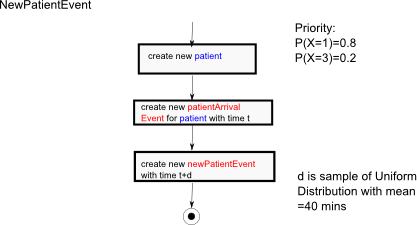
\includegraphics{img/NewPatientEvent}
  	\caption{New Patient Event}
\end{figure}

\subsection{Busy/Free Doctor Warteschlangen}
Die Doktoren in unserer Notaufnahme werden mittels zwei Warteschlangen verwaltet. Diese Graphik beschreibt den Statuswechsel der Doktoren.
%\frametitle{Busy/Free Doctor}
\begin{center}
%  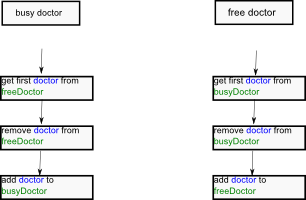
\includegraphics{img/freeDoctor}
\end{center}

\newpage
\subsection{Patient Arrival Event}
\textit{Patient Arrival Event} modelliert die Ankunft eines Patienten.
Abh\"{a}ngig von der Priorit\"{a}t des Patienten wird dieser in einer der 3 Warteschlangen gegeben. Wurde der Patient im Sinne unserer Erweiterung von einem Patienten mit Priorit\"{a}t 3 abgel\"{o}\ss t dh. wurde seine Behandlung durch einen Priorit\"{a}t 3 abgebrochen, wird dieser in vorne in die Warteschlange seiner Priorit\"{a}t eingereiht. Handelt es sich bei dem Patienten um einen Patienten der Priorit\"{a}t 3 wird f\"{u}r diesen weiter die Zeitpunkt seines Todes bestimmt. (\textit{Patient Death Event})
Abh\"{a}ngig davon, ob ein Doktor frei ist (dh. gerade keinen Patienten behandelt) oder nicht, wird der Patient einem Doktor zugewiesen oder aber er verbleibt in der Warteschlange.
Handelt es sich beim Patienten um einen Notfall hat dieser auch wenn kein Doktor frei sein sollte durch Abl\"{o}sung eines sich in Behandlung befindlichen Priorit\"{a}t 1 Patienten die M\"{o}glichkeit sofort behandelt zu werden.


\begin{figure}[h]
	\centering
%	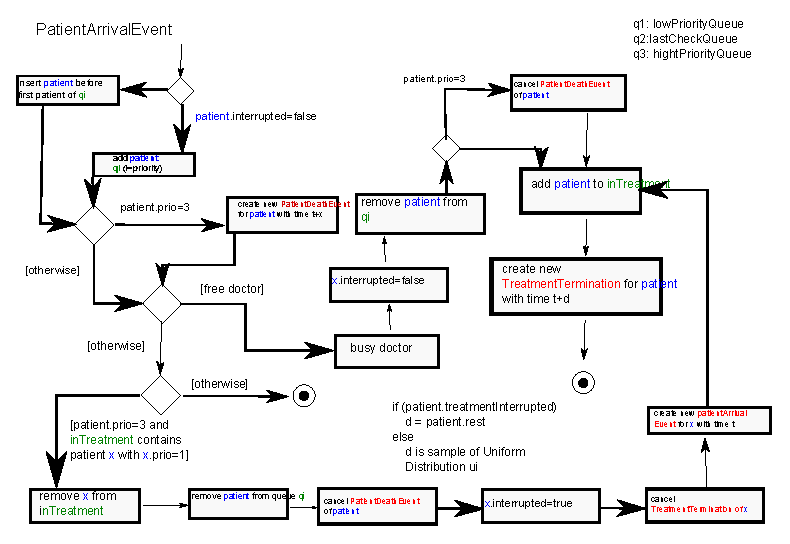
\includegraphics{img/PatientArrivalEvent}
	\caption{Patient Arrival Event}
\end{figure}


\newpage

\subsection{Treatment Termination Event}
\textit{Treatment Termination Event} ist sowhol auschlaggebend f\"{u}r den weiteren Verlauf des Patienten in der Notaufnahme, als auch f\"{u}r die Dauer seiner Behandlung. Der Patient wird aus der Behandlungswarteschlange genommen. Ist dessen Priorit\"{a}t nicht 2 (sondern 3 oder 1), dann wird seine Priorit\"{a}t auf 2 gesetzt und anschlie\ss end ein \textit{Patient Arrival Event} f\"{u}r diesen erstellt. Ist jedoch seine Priorit\"{a}t 2, so verl\"{a}sst er die Notaufnahme.
Beinhalten nun alle Warteschlangen der Patienten keine Patienten, so wird der Doktor (der diesen Patienten behandelte) auf verf\"{u}gbar gesetzt, in dem er der \textit{Free Doctor Warteschlange} hinzugef\"{u}gt wird. Enth\"{a}lt jedoch eine der Patienten Warteschlangen einen Patienten (\"{U}berpr\"{u}fung erfolgt absteigend (3,2,1)),  so wird dieser aus der Warteschlange entfernt und wird von einem Doktor behandelt (Hinzuf\"{u}gen der \textit{Treatement Warteschlange}). Ebenso wird ein neues \textit{Treatement Termination} Event f\"{u}r den neuen Patienten mit einer Behandlungszeit erstellt und der Ereignisliste hinzugef\"{u}gt.
Hat dieser neue Patient eine Priorit\"{a}t von 3, so wird sein \textit{Patient Death Event}, welches den Tod f\"{u}r diesen nicht behandelten akuten Notfall darstellt, abgebrochen.

\begin{figure}[h]
	\centering
	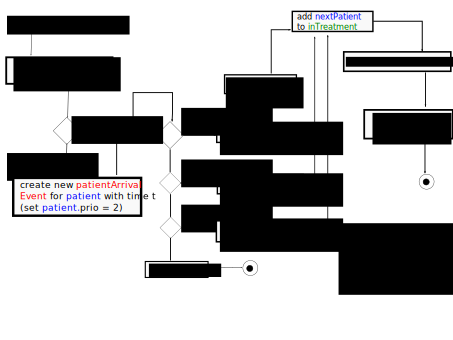
\includegraphics{img/TreatmentTermination}
	\caption{Treatment Termination Event}
\end{figure}





\newpage

\section{Ergebnisse}
Im Folgenden sollen die Ergebnisse, welche das Resultat von jeweils hundert Simulationsl\"{a}ufen sind, einer n\"{a}heren Betrachtung unterzogen werden.
Wie in \ref{sec:Aufgabe} beschrieben, war es Teil der Aufgabenstellung die Simulation mit und ohne Initialisierungsphase durchzuf\"{u}hren.
Desweiteren haben wir die Auswirkung  der von uns erdachten Erweiterungen betrachtet und analysiert.
Folgende Ergebnisgr\"{o}{\ss}en waren f\"{u}r uns von besonderem Interesse:
\begin{itemize}

	\item mittlerer Wartezeit beider Patientenarten\newline
	Die mittlere Wartezeit der Patienten nimmt mit einer zunehmenden Anzahl an Doktoren ab.
	Weiters konnten wir durch die Notfall-Priorit\"{a}t die mittlere Wartezeit der Priorit\"{a}t 3 Patienten um 50\% verk\"{u}rzen. Dies f\"{u}hrte zu eine
	Verringerung der Tode um etwa 40\%. Gleichzeitig f\"{u}hrte die Notfallpriorit\"{a}t zu einem 10\% Anstieg der mittleren Wartezeit der Priorit\"{a}t 1 und Priorit\"{a}t 2 Patienten. 
	
	\item Anteil der Patienten die nicht warten/maximal 5 Minuten warten m\"{u}ssen.\newline
	Die Anzahl der Patienten, welche maximal 5 Minuten warten mussten nahm erwartungsgem\"{a}{\ss} mit der Anzahl der Doktoren zu und erreichte bei 5 Doktoren ihr Maximum. Eine vorgeschaltete Initialisierungsphase f\"{u}hrt zu einer Verminderung des Anteils solcher Patienten.
Eine Initialisierungsphase sorgt daf\"{u}r, dass die Warteschlangen zu Begin der eigentlichen Simulation nicht leer sind bzw.
 die Behandlungsr\"{a}ume der Doktoren besetzt sind. Daraus resultiert nat\"{u}rlich ein gr\"{o}{\ss}erer Anteil an Patienten mit einer Wartezeit von \"{u}ber 5 Minuten. 
	Der Anteil der Patienten, welche gar nicht warten mussten verhielt sich bez\"{u}glich der Anzahl der Doktoren und Initialisierungsphase gleicherma{\ss}en.

	\item Zeit x, welche 90\% der Patienten in der Notaufnahme verbracht haben \newline
	Auch hier konnte erwartungsgem\"{a}{\ss} eine Abnahme der Wartezeit mit zunehmender Anzahl an Doktoren beobachtet werden. Bei 4 Doktoren entsprach die Zeit x schon in etwa der durchschnittlichen Behandlungszeit der Patienten. 
Eine Initialisierungsphase f\"{u}hrte zu einer h\"{o}hren Zeit.

	\item maximale und mittlere Anzahl der wartenden akuten Notf\"{a}lle und restlichen Patienten \newline
	Wie die mittlere Wartezeit nimmt auch die mittlere Anzahl der wartenden Patienten mit einer Zunahme der Anzahl an Doktoren ab. Selbiges gilt f\"{u}r die maximale Anzahl von Patienten in der Warteschlange. Eine vorgeschaltete Initialisierungsphase erh\"{o}ht sowohl die mittlere als auch maximale Anzahl der Patienten in der Warteschlange.
Das Konzept der Notfallpriorit\"{a}t f\"{u}hrt erwartungsgem\"{a}{\ss} zu einer Verminderung der mittleren und maximalen Anzahl an wartenden Patienten der Priorit\"{a}t 3 Patienten.
	
\end{itemize}





\end{document}






